\documentclass[10pt]{article}
\usepackage{graphicx}
\usepackage[none]{hyphenat}
\usepackage{graphicx}
\usepackage{listings}
\usepackage[english]{babel}
\usepackage{siunitx}
\usepackage{graphicx}
\usepackage{caption} 
\usepackage{booktabs}
\usepackage{array}
\usepackage{amssymb} % for \because
\usepackage{amsmath}   % for having text in math mode
\usepackage{extarrows} % for Row operations arrows
\usepackage{listings}
\usepackage[utf8]{inputenc}
\lstset{
  frame=single,
  breaklines=true
}
\usepackage{hyperref}
  
%Following 2 lines were added to remove the blank page at the beginning
\usepackage{atbegshi}% http://ctan.org/pkg/atbegshi
\AtBeginDocument{\AtBeginShipoutNext{\AtBeginShipoutDiscard}}


%New macro definitions
\newcommand{\mydet}[1]{\ensuremath{\begin{vmatrix}#1\end{vmatrix}}}
\providecommand{\brak}[1]{\ensuremath{\left(#1\right)}}
\newcommand{\solution}{\noindent \textbf{Solution: }}
\newcommand{\myvec}[1]{\ensuremath{\begin{pmatrix}#1\end{pmatrix}}}
\providecommand{\norm}[1]{\left\lVert#1\right\rVert}
\providecommand{\abs}[1]{\left\vert#1\right\vert}
\let\vec\mathbf{}
\begin{document}

\begin{center}
\title{\textbf{STRAIGHT LINES}}
\date{\vspace{-5ex}} %Not to print date automatically
\maketitle
\end{center}

\section{11$^{th}$ Maths - Chapter 10}
This is Problem 11 from Exercise-10.3
\begin{enumerate}
\item Prove that the line through the point$(x_1,y_1)$ and parallel to the line A$x$+B$y$+C=0 is A$(x-x_1)$+B$(y-y_1)$=0.

\solution
Given 
\begin{align}
\text{ Let }\vec{P}=\myvec{x_1\\y_1}\\
Ax+By+C=0
\label{eq1}
\end{align}
The line equation is
\begin{align}
\vec{n}^{\top}\vec{x}=c
\end{align}
from \eqref{eq1}

\begin{align}
\vec{n}=\myvec{A\\B}
\end{align}
The line passing through the $\vec{P}$ is parallel to line $Ax+By+C=0$.\\
The line equation for line passing through $\vec{P}$ is
\begin{align}
\vec{n}^{\top}\vec{m}=0\\
\vec{n}^\top\brak{\vec{x}-\vec{P}}=0\\
\myvec{A&B}\brak{\myvec{x\\y}-\myvec{x_1\\y_1}}=0\\
\myvec{A&B}\myvec{x-x_1\\y-y_1}=0\\
A(x-x_1)+B(y-y_1)=0
\end{align}
\begin{figure}[!h]
	\begin{center}
		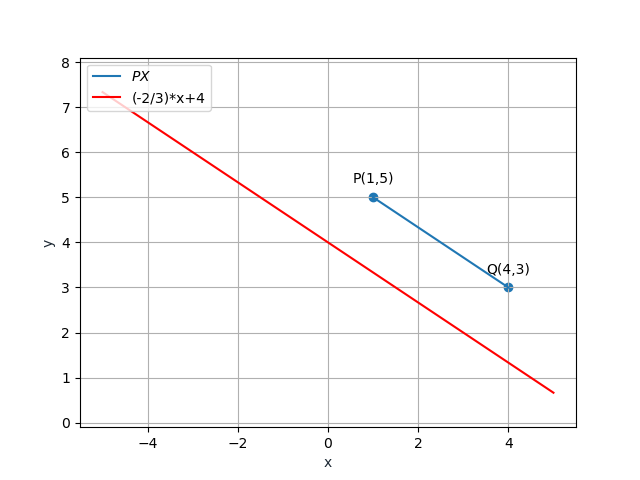
\includegraphics[width=\columnwidth]{./figs/fig.png}
	\end{center}
\caption{}
\end{figure}

\end{enumerate}
\end{document}
